\input ../SlidePreamble
\input ../preamble


\begin{document}

{\Huge


\centerline{\bf TTIC 31230, Fundamentals of Deep Learning}
\bigskip
\centerline{David McAllester, Winter 2020}

\vfill
\centerline{\bf PAC-Bayesian Learning Theory}
\vfill
\vfill

\slide{Chomsky vs. Kolmogorov and Hinton}

\includegraphics[width=1.0 in]{../images/Chomsky} \begin{minipage}[b]{8in} Noam Chomsky: 
Natural language grammar cannot be learned by a universal learning algorithm.
This position is supported by the ``no free lunch theorem''.\end{minipage}

\vfill
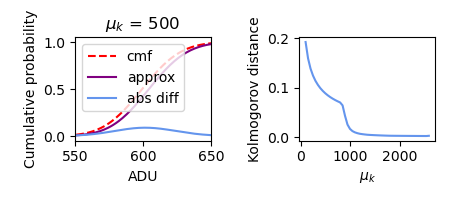
\includegraphics[height=1.0 in]{../images/Kolmogorov}
\includegraphics[height=1.0 in]{../images/Hinton}
\begin{minipage}[b]{7in}
Andrey Kolmogorov, Geoff Hinton: Universal learning algorithms exist. This position is supported by the ``free lunch theorem''.
\end{minipage}

\slide{The No Free Lunch Theorem}

\includegraphics[width=1.0 in]{../images/Chomsky} 

Without prior knowledge, such as universal grammar, it is impossible to make a prediction for an input you have not seen in the training data.


\vfill
{\bf Proof:} Select a predictor $h$ uniformly at random from all functions from ${\cal X}$ to ${\cal Y}$ and then take the data distribution to draw pairs $(x, h(x))$
where $x$ is drawn uniformly from ${\cal X}$.  No learning algorithm can predict $h(x)$ where $x$ does not occur in the training data.


\slide{The Free Lunch Theorem}

Consider a classifier $f$ written in C++ with an arbitrarily large standard library.

\vfill
Let $|f|$ be the number of bits needed to represent $f$.

\slide{The Free Lunch Theorem}

\vfill
$$0 \leq {\cal L}(h,x,y) \leq \lmax$$
\begin{eqnarray*}
{\cal L}(h)  & = &  E_{(x,y)\sim \mathrm{Pop}}\;{\cal L}(h,x,y) \\
\hat{{\cal L}}(h) & = & E_{(x,y)\sim \mathrm{Train}}\;{\cal L}(h,x,y)
\end{eqnarray*}

\vfill
Theorem: With probability at least $1-\delta$ over the draw of the training data the following holds simultaneously for all $f$.

{\color{red} $$E(f) \leq \frac{10}{9}\left(\hat{E}(f) + \frac{5\lmax}{N_\mathrm{Train}}\left((\ln 2)|f| +\ln\frac{1}{\delta}\right)\right)$$}


\slide{Free Lunch Theorem (Probability Form)}

Code length is inter-convertable with with probability.

$$P(h) = 2^{-|h|}\;\;\;\mbox{or}\;\;\;|h| = - \log_2 P(h)$$

\vfill
Instead of fixing the language (e.g., C++ with a large library) we fix a prior $P(h)$.

\vfill
    {\bf Theorem:} With probability
    at least $1-\delta$ over the draw of training data the following holds simultaneously for all $h$.

\vfill
    $${\cal L}(h) \leq \frac{10}{9}\parens{\hat{\cal L}(h) + \frac{5 L_\mathrm{max}}{N_\mathrm{Train}}\parens{\ln \frac{1}{P(h)} + \ln\frac{1}{\delta}}}$$

\slide{Proof}

Define
$$\epsilon(h) = \sqrt{\frac{2{\cal L}(h)\parens{\ln\frac{1}{P(h)} + \ln\frac{1}{\delta}}}{\lmax N_\mathrm{Train}}}.$$

\vfill
By the relative Chernov bound we have

\vfill
$$P_{\mathrm{Train} \sim \mathrm{Pop}}\parens{\frac{\hat{{\cal L}}(h)}{\lmax} \leq \frac{{\cal L}(h)}{\lmax} - \epsilon(h)} \leq e^{-N_\mathrm{Train}\frac{\epsilon(h)^2\lmax}{2{\cal L}(h)}} = \delta P(h).$$

\slide{Proof}

$$P_{\mathrm{Train} \sim \mathrm{Pop}}\parens{\hat{{\cal L}}(h) \leq {\cal L}(h) - \lmax\epsilon(h)} \leq \delta P(h).$$

\vfill
$$P_{\mathrm{Train} \sim \mathrm{Pop}}\parens{\exists h\;\hat{{\cal L}}(h) \leq {\cal L}(h) - \lmax\epsilon(h)} \leq \sum_h \delta P(h) =\delta$$

\vfill
$$P_{\mathrm{Train} \sim \mathrm{Pop}}\parens{\forall h\;{\cal L}(h) \leq \hat{{\cal L}}(h) + \lmax\epsilon(h)} \geq 1- \delta$$

\slide{Proof}

$${\cal L}(h) \leq \widehat{{\cal L}}(h) + \lmax\sqrt{\frac{{\cal L}(h)}{\lmax}\parens{\frac{2\parens{\ln\frac{1}{P(h)} + \ln\frac{1}{\delta}}}{N_\mathrm{Train}}}}$$

using
$$\sqrt{ab} = \inf_{\lambda > 0}\;\frac{a}{2\lambda} + \frac{\lambda b}{2}$$
\vfill
we get
$${\cal L}(h) \leq \widehat{{\cal L}}(h) + \frac{{\cal L}(h)}{2\lambda} + \frac{\lambda\lmax\parens{\ln\frac{1}{P(h)} + \ln\frac{1}{\delta}}}{N_\mathrm{Train}}$$

\slide{Proof}
$${\cal L}(h) \leq \widehat{{\cal L}}(h) + \frac{{\cal L}(h)}{2\lambda} + \frac{\lambda\lmax\parens{\ln\frac{1}{P(h)} + \ln\frac{1}{\delta}}}{N_\mathrm{Train}}$$

\vfill
Solving for ${\cal L}(h)$ yields

\vfill
$${\cal L}(h) \leq \frac{1}{1-\frac{1}{2\lambda}}\parens{\hat{{\cal L}}(h) + \frac{\lambda\lmax}{N_\mathrm{Train}}\parens{\ln \frac{1}{P(h)} + \ln \frac{1}{\delta}}}$$

\vfill
Setting $\lambda = 5$ brings the leading factor to 10/9 which seems sufficiently close to 1 that larger values of $\lambda$ need not be considered.

\slide{A Model Compression Guarantee}

Let $|\Phi|$ be the number of bits used to represent $\Phi$ under some fixed compression scheme.

\vfill
Let $P(\Phi) = 2^{-|\Phi|}$

\vfill
    $${\cal L}(\Phi) \leq \frac{10}{9}\parens{\hat{\cal L}(\Phi) + \frac{5 L_\mathrm{max}}{N_\mathrm{Train}}\parens{(\ln 2)|\Phi| + \ln\frac{1}{\delta}}}$$


\slide{A Bound for Continuous Densities}

Let $p$ be any ``prior'' and $q$ be any ``posterior'' on any  (possibly continuous) model space.
Define
\begin{eqnarray*}
  L(q) & =  &\expectsub{h \sim q}{L(h)} \\
  \\
  \hat{L}(q) & =  &\expectsub{h \sim q}{\hat{L}(h)}
\end{eqnarray*}


\vfill
For any $p$ and any $\lambda > \frac{1}{2}$, with probability
at least $1-\delta$ over the draw of the training data, the following holds simultaneously for all $q$.
\vfill
$$L(q) \leq \frac{1}{1-\frac{1}{2\lambda}}\parens{\hat{L}(q) + \frac{\lambda \lmax}{N_\mathrm{Train}}\parens{KL(q,p) + \ln \frac{1}{\delta}}}$$

\slide{Adding Noise Simulates Limiting Precision}

Assume $0 \leq {\cal L}(\Phi,x,y) \leq \lmax$.

\vfill
Define:
\begin{eqnarray*}
{\cal L}(\Phi) & = & E_{\;(x,y)\sim \pop,\;\epsilon \sim {\cal N}(0,\sigma)^d}\;{{\cal L}(\Phi+\epsilon,x,y)} \\
\\
\hat{{\cal L}}(\Phi) & = & E_{\;(x,y)\sim \mathrm{Train},\;\epsilon \sim {\cal N}(0,\sigma)^d}\;{{\cal L}(\Phi+\epsilon,x,y)} \\
\end{eqnarray*}

\vfill
Theorem: With probability at least $1-\delta$ over the draw of training data the following holds {\bf simultaneously} for all $\Phi$.
\begin{eqnarray*}
   {\color{red} {\cal L}(\Phi)} & {\color{red} \leq} & {\color{red} \frac{10}{9}\parens{\hat{{\cal L}}(\Phi)
   + \frac{5 \lmax}{N_\mathrm{Train}}\parens{\frac{||\Phi-\Phi_{\mathrm{init}}||^2}{2\sigma^2} + \ln \frac{1}{\delta}}}}
\end{eqnarray*}

\slide{Non-Vacuous Generalization Guarantees}

Model compression has recently been used to achieve ``non-vacuous'' PAC-Bayes generalization guarantees for ImageNet classification
--- error rate guarantees less than 1.

\vfill
Non-Vacuous PAC-Bayes Bounds at ImageNet Scale.

\bigskip
Wenda Zhou, Victor Veitch, Morgane Austern, Ryan P. Adams, Peter Orbanz

\bigskip
ICLR 2019

\slide{END}

}
\end{document}
